% ══════════════════════════════════════════════════════════════════════
% EMPIRICAL RESULTS — AGENT × TENANT EVALUATION
% Input this file inside \section{Experiments}, after \subsection{Experimental Setup}
% ══════════════════════════════════════════════════════════════════════

\subsubsection{Agent Configurations}
\label{sec:agent-configs}

We evaluate three agent configurations whose designs span a spectrum from minimal reactive reasoning to deliberative multi-step planning. All three share the same embedding model (\texttt{text-embedding-ada-002}) and use GPT-4o-family models via Azure OpenAI: the two ReAct agents use GPT-4o while the Researcher agent uses GPT-4o-mini. This design varies architecture, prompt engineering, and model size simultaneously, reflecting the realistic design space in which practitioners choose agent configurations.

\begin{table}[h]
\centering
\caption{Configuration summary for the three evaluated agents.
``Planning model'' refers to the LLM used for the optional pre-execution planning step.
Prompt size is the approximate system-prompt token count. Avg.\ tool calls and latency are empirical means across all evaluation cases.}
\label{tab:agent_configs}
\small
\begin{tabular}{p{0.12\linewidth}p{0.12\linewidth}p{0.12\linewidth}p{0.06\linewidth}p{0.10\linewidth}p{0.10\linewidth}p{0.10\linewidth}p{0.10\linewidth}}
\toprule
\textbf{Agent} & \textbf{Architecture} & \textbf{Model} & \textbf{$T$} & \textbf{Planning Model} & \textbf{Prompt Size} & \textbf{Avg.\ Tools} & \textbf{Avg.\ Lat.\ (s)} \\
\midrule
\textsc{ReAct-v1}   & Single-pass ReAct & GPT-4o      & 0.7 & ---               & $\sim$3k tok   & 1.70 & 17.6 \\
\textsc{ReAct-v2}   & Single-pass ReAct & GPT-4o      & 0.5 & ---               & $\sim$1.5k tok & 1.70 & 18.2 \\
\textsc{Researcher}  & Plan\,+\,Execute  & GPT-4o-mini & 0.0 & GPT-4o-mini ($T{=}0$) & $\sim$3k tok   & 4.85 & 65.2 \\
\bottomrule
\end{tabular}
\end{table}

\textsc{ReAct-v1} implements a standard ReAct loop~\cite{yao2022react} with a verbose system prompt ($\sim$3{,}000 tokens) containing eight fully worked \textsc{Thought}$\to$\textsc{Tool} examples. These examples concretely demonstrate several critical behavioral patterns: dual-term person lookup (searching simultaneously by display name and by user~ID), pronoun-to-ID resolution before issuing any content search, multi-query decomposition for relationship-based questions (``emails between A and B''), and detailed citation formatting with per-fact inline superscripts and a mandatory \texttt{\#\# References} section listing artifact IDs. Its execution temperature of 0.7 permits exploratory variation in search-query phrasing.

\textsc{ReAct-v2} shares the same single-pass ReAct loop but condenses the system prompt to $\sim$1{,}500 tokens across five terse bullet-style examples. The instructions cover the same topics---people resolution, citation formatting, pronoun disambiguation---but omit the extended worked demonstrations, replacing them with one-line directives. Its execution temperature is lowered to 0.5.

\textsc{Researcher} introduces a dedicated planning stage: GPT-4o-mini (at temperature~0.0) first generates a structured, step-by-step research plan before any tool call is issued. The planning prompt explicitly requires four capabilities: (i)~\emph{multi-hop reasoning}---decomposing complex questions into dependency chains; (ii)~\emph{correlated search}---cross-referencing across emails, chats, meetings, and files; (iii)~\emph{mandatory ID resolution}---resolving names to user IDs via \texttt{search\_people} before any content search; and (iv)~\emph{step-by-step ordering}---arranging steps so that the output of each feeds the next. The planner is instructed to output only the plan, not to execute it. The same GPT-4o-mini model (at temperature~0.0) then executes the plan step by step using the full tool set, resulting in systematically broader retrieval (61.6 items retrieved per case vs.\ 15--19 for the reactive agents) and substantially higher token consumption ($\sim$92k prompt tokens vs.\ $\sim$18k). Notably, despite using a smaller model than the ReAct agents, the Researcher achieves the highest pass rate, demonstrating that structured planning can compensate for reduced per-call model capacity.

\subsubsection{Evaluation Metrics}
\label{sec:eval-metrics}

Each evaluation case consists of a natural-language query, a requesting user identity, a list of gold-standard factual assertions, and a list of entity references that a correct answer should cite. Three query generators produce cases of increasing complexity:

\begin{enumerate}[leftmargin=*,nosep]
\item \textbf{Search queries} target the retrieval of specific items with filtering constraints (e.g., ``Find emails sent by Lisa about fund Beta in the last two weeks'').
\item \textbf{Multi-hop queries} require chaining evidence across artifact types and resolving entity relationships (e.g., ``Who attended the meeting where the Q3 budget was discussed, and what follow-up action did they take by email?'').
\item \textbf{Report queries} request synthesis or summary generation over multi-day windows (e.g., ``Provide a timeline of all decisions related to the server migration from March 1 to March 15'').
\end{enumerate}

\noindent The automated judge (GPT-4o, temperature~0.0) computes four complementary metrics via separate LLM calls:

\paragraph{Assertion score.} Each gold assertion $a_i$ is verified independently against the agent's response. The judge outputs a Boolean \emph{True}/\emph{False} per assertion together with a brief explanation, and the final assertion score for the case is the fraction of assertions satisfied: $\text{Assr.} = |\{a_i : \text{True}\}| / |A|$.

\paragraph{Tool-search relevance.} The judge evaluates three aspects of the agent's tool usage in a single call: (i)~whether the tool calls were \emph{appropriate} for the query, (ii)~whether the retrieved evidence was \emph{relevant} to the question, and (iii)~whether the final response is \emph{grounded} in the retrieved artifacts rather than hallucinated. The result is a scalar relevance score in $[0,1]$. We additionally record the number of items retrieved per case (\emph{tool-search count}).

\paragraph{Response-citation quality.} A separate judge call inspects the response's \texttt{\#\# References} section, checking (i)~whether one exists, (ii)~how many cited artifact IDs are \emph{grounded} (i.e., appear in the tool-call results) versus \emph{hallucinated} (fabricated IDs), and (iii)~whether inline citation markers appear in the response body. The score is in $[0,1]$; we also record the raw grounded-citation count.

\paragraph{Pass rate.} A case is marked \emph{passed} if the assertion score is~1.0 (all assertions satisfied). Pass rate is the fraction of cases that pass.

\noindent For aggregate reporting, we define a composite \emph{citation score} as the mean of tool-search relevance and response-citation quality. This decomposition is important because the two sub-scores measure different failure modes: an agent can retrieve excellent evidence but fail to format citations (high tool-search, low response-citation), or it can produce well-formatted references that point to irrelevant material (low tool-search, high response-citation).

\subsubsection{Main Results}
\label{sec:main-results}

Table~\ref{tab:results_full} reports the decomposed metrics across all nine agent--tenant combinations. Table~\ref{tab:agent_ranking} aggregates results across tenants.

\begin{table}[h]
\centering
\caption{Per-tenant and per-agent evaluation results.
\emph{Pass}: pass rate. \emph{Assr.}: assertion score. \emph{TS-Rel}: tool-search relevance. \emph{TS-$n$}: mean items retrieved. \emph{RC-Rel}: response-citation relevance. \emph{RC-$n$}: mean grounded citations. \emph{Cite}: composite citation score (mean of TS-Rel and RC-Rel). \emph{Lat.}: mean latency in seconds.
Bold marks the best per-tenant value.}
\label{tab:results_full}
\resizebox{\linewidth}{!}{%
\begin{tabular}{llcccccccc}
\toprule
\textbf{Tenant} & \textbf{Agent} & \textbf{Cases} & \textbf{Pass} & \textbf{Assr.} & \textbf{TS-Rel} & \textbf{TS-$n$} & \textbf{RC-Rel} & \textbf{Cite} & \textbf{Lat.\ (s)} \\
\midrule
\multirow{3}{*}{Bertrand}
  & \textsc{ReAct-v1}   & 162 & 0.414              & \textbf{0.736} & \textbf{0.803} & 19.2 & 0.593              & 0.698              & \textbf{18.1} \\
  & \textsc{ReAct-v2}   & 162 & 0.259              & 0.729          & 0.650          & 15.8 & 0.479              & 0.565              & 22.2 \\
  & \textsc{Researcher}  & 162 & \textbf{0.432}     & 0.625          & 0.762          & \textbf{61.1} & \textbf{0.640}     & \textbf{0.701}     & 71.0 \\
\midrule
\multirow{3}{*}{Cambford}
  & \textsc{ReAct-v1}   & 162 & 0.228              & \textbf{0.515} & 0.717          & 18.3 & 0.449              & 0.583              & 17.3 \\
  & \textsc{ReAct-v2}   & 162 & 0.222              & 0.489          & 0.701          & 17.0 & 0.440              & 0.571              & \textbf{15.8} \\
  & \textsc{Researcher}  & 162 & \textbf{0.346}     & 0.543          & \textbf{0.793} & \textbf{61.1} & \textbf{0.684}     & \textbf{0.738}     & 55.3 \\
\midrule
\multirow{3}{*}{ZAI}
  & \textsc{ReAct-v1}   & 201 & 0.269              & \textbf{0.560} & \textbf{0.797} & 17.9 & 0.558              & \textbf{0.677}     & \textbf{19.1} \\
  & \textsc{ReAct-v2}   & 201 & 0.154              & 0.473          & 0.717          & 13.5 & 0.493              & 0.605              & 16.5 \\
  & \textsc{Researcher}  & 201 & \textbf{0.289}     & 0.503          & 0.765          & \textbf{62.5} & \textbf{0.623}     & 0.694              & 69.1 \\
\bottomrule
\end{tabular}
}
\end{table}

\begin{table}[h]
\centering
\caption{Aggregate agent rankings across all three tenants.
Columns follow the same conventions as Table~\ref{tab:results_full}.
\emph{Prompt tok.}: mean input tokens per inference call. \emph{Tool calls}: mean tool invocations per case.}
\label{tab:agent_ranking}

\begin{figure}[h]
\centering
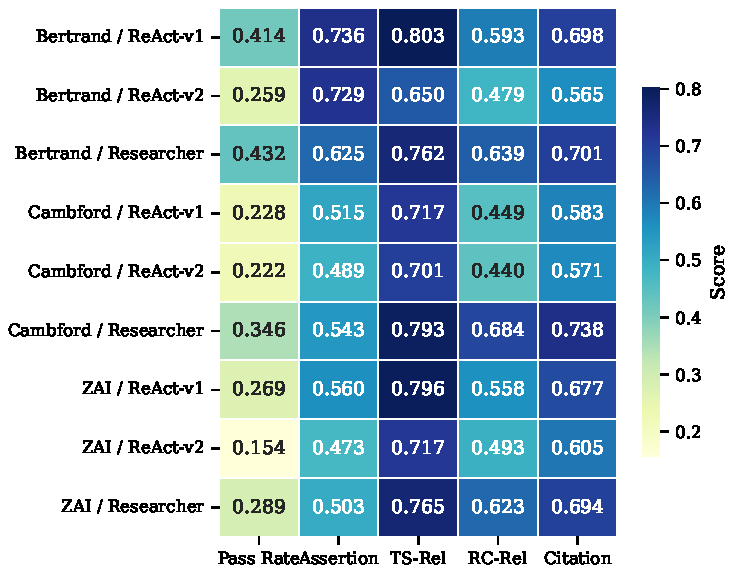
\includegraphics[width=0.9\linewidth]{figures/metrics_heatmap.pdf}
\caption{Evaluation metrics heatmap across all nine agent--tenant combinations. Darker cells indicate higher values. The heatmap provides a compact visual summary of the strengths and weaknesses of each agent configuration across tenants and metric dimensions.}
\label{fig:metrics_heatmap}
\end{figure}

\small
\begin{tabular}{lcccccccccc}
\toprule
\textbf{Agent} & \textbf{Pass} & \textbf{Assr.} & \textbf{TS-Rel} & \textbf{TS-$n$} & \textbf{RC-Rel} & \textbf{RC-$n$} & \textbf{Cite} & \textbf{Lat.\ (s)} & \textbf{Tools} & \textbf{Prompt tok.} \\
\midrule
\textsc{Researcher}  & \textbf{0.355} & 0.557          & 0.773          & \textbf{61.6} & \textbf{0.649} & \textbf{2.81} & \textbf{0.711} & 65.2          & \textbf{4.85} & 92{,}280 \\
\textsc{ReAct-v1}   & 0.323          & \textbf{0.638} & \textbf{0.799} & 18.5          & 0.551          & 1.87          & 0.675          & \textbf{17.6} & 1.70          & 17{,}778 \\
\textsc{ReAct-v2}   & 0.212          & 0.564          & 0.689          & 15.4          & 0.471          & 1.84          & 0.580          & 18.2          & 1.70          & 17{,}203 \\
\bottomrule
\end{tabular}
\end{table}

\begin{figure}[h]
\centering
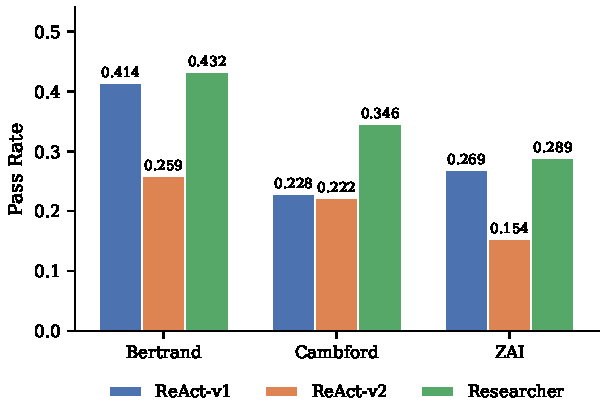
\includegraphics[width=0.9\linewidth]{figures/pass_rate_by_agent_tenant.pdf}
\caption{Pass rate (fraction of cases with all assertions satisfied) by agent configuration and tenant. \textsc{Researcher} leads on Bertrand and Cambford; the gap narrows on ZAI where evidence is temporally concentrated.}
\label{fig:pass_rate}
\end{figure}

\begin{figure}[h]
\centering
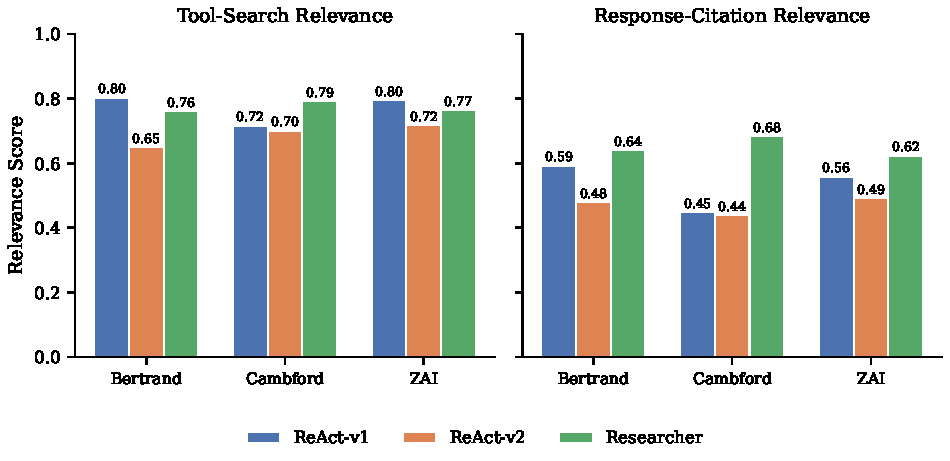
\includegraphics[width=0.9\linewidth]{figures/citation_decomposition.pdf}
\caption{Decomposed citation metrics. \textsc{ReAct-v1} leads on tool-search relevance (left) while \textsc{Researcher} leads on response-citation quality (right), showing that retrieval precision and citation formatting are largely independent failure modes.}
\label{fig:citation_decomp}
\end{figure}

\begin{figure}[h]
\centering
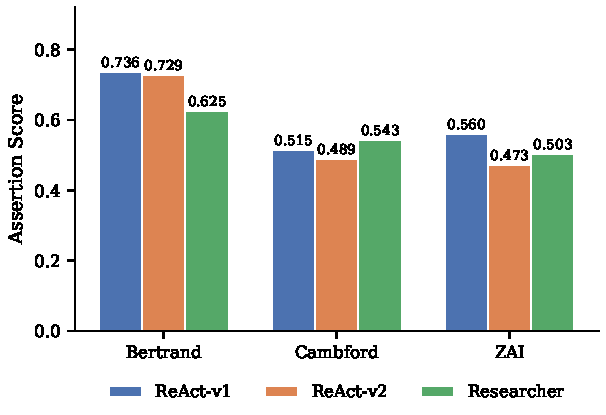
\includegraphics[width=0.9\linewidth]{figures/assertion_score_by_agent_tenant.pdf}
\caption{Mean assertion score (fraction of gold assertions satisfied) by agent and tenant. \textsc{ReAct-v1} leads on factual precision across all three tenants, while \textsc{Researcher}'s broad retrieval strategy sacrifices per-assertion accuracy for coverage.}
\label{fig:assertion_score}
\end{figure}

\noindent \textsc{Researcher} achieves the highest overall pass rate (35.5\%) and citation quality (0.711) but the lowest assertion score (0.557). \textsc{ReAct-v1} ranks second on pass rate (32.3\%) while leading on assertion accuracy (0.638) and tool-search relevance (0.799). \textsc{ReAct-v2} trails on all quality metrics (pass 21.2\%, citation 0.580) despite its structural similarity to v1. The decomposed citation scores reveal that \textsc{Researcher}'s advantage is concentrated in response-citation quality (0.649 vs.\ 0.551 for v1), while \textsc{ReAct-v1} actually leads on tool-search relevance (0.799 vs.\ 0.773). This means that the reactive agent retrieves slightly more relevant evidence per tool call, but the planning agent produces better-structured reference sections because its broader retrieval footprint provides more citable material.

\subsubsection{Effect of Agent Architecture: Plan-and-Execute vs.\ ReAct}
\label{sec:arch-analysis}

The primary architectural difference between \textsc{Researcher} and the two reactive agents is the separation of planning from execution. Before issuing any tool call, \textsc{Researcher} prompts GPT-4o-mini to produce a structured research plan that decomposes the query into a dependency chain, identifies which data modalities to cross-reference, and mandates people-ID resolution before any content search. This design directly explains three empirical patterns.

First, \textsc{Researcher} retrieves 61.6 items per case versus 15--19 for the reactive agents---a factor of $\sim$3.5$\times$. The planning prompt explicitly requires correlated search across emails, chats, meetings, and files, whereas the reactive agents only pursue additional artifact types opportunistically. This broader retrieval footprint is the primary driver of the response-citation advantage: with more retrieved artifacts available, the execution model has more material to cite, raising the grounded-citation count from 1.87 (v1) to 2.81 (\textsc{Researcher}).

\begin{figure}[h]
\centering
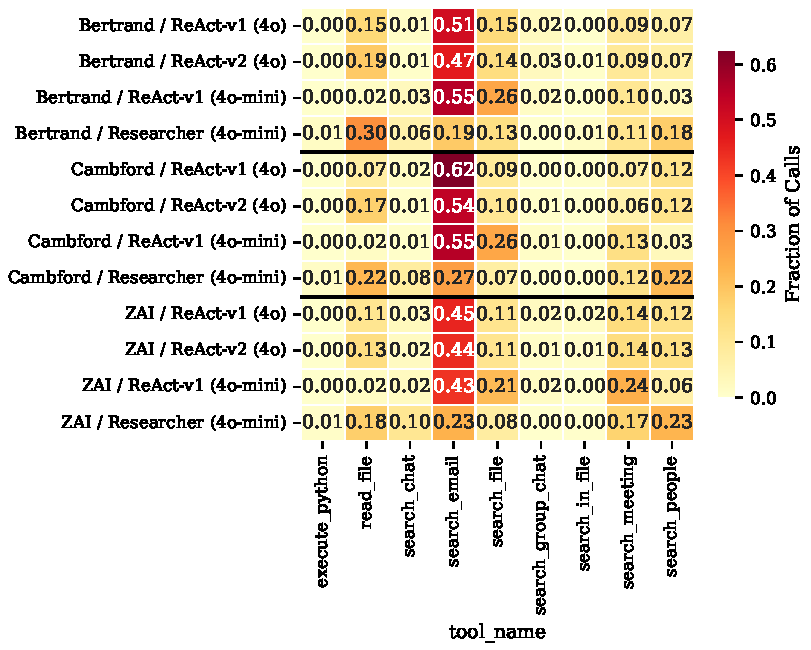
\includegraphics[width=0.9\linewidth]{figures/tool_usage_heatmap.pdf}
\caption{Tool-call distribution by agent and tenant. Rows are grouped by tenant; columns show individual tools. \textsc{Researcher} allocates calls across more tool types in every tenant, while the reactive agents concentrate on \texttt{search\_messages} and \texttt{search\_people}. Cross-tenant variation is visible: ZAI's larger corpus drives higher \texttt{read\_file} usage across all agents.}
\label{fig:tool_usage}
\end{figure}

Second, the planning stage is most beneficial when queries require temporal multi-hop reasoning. On Cambford, where cases frequently require reconstructing policy evolution across weeks of committee emails and subsequent meeting threads, \textsc{Researcher} improves pass rate by 52\% relative to \textsc{ReAct-v1} (0.346 vs.\ 0.228) and achieves the highest citation score in any cell (0.738). On Bertrand, where the smaller, denser organization makes most answers reachable via a single well-formed search, the pass-rate gap shrinks to 4\% (0.432 vs.\ 0.414). On ZAI, where evidence is concentrated in dense operational bursts, \textsc{ReAct-v1} closes to within 2 percentage points of \textsc{Researcher} on pass rate (0.269 vs.\ 0.289) and substantially exceeds it on assertion score (0.560 vs.\ 0.503).

Third, despite leading on pass rate and citation, \textsc{Researcher} lags on assertion score (0.557 vs.\ 0.638 for v1). Two factors contribute: the smaller GPT-4o-mini model has lower per-call reasoning capacity than GPT-4o, and the deterministic $T{=}0.0$ decoding constrains the model's ability to flexibly integrate retrieved evidence into cohesive factual statements. The planning stage further compounds this by guiding execution toward broad retrieval at the expense of precise fact synthesis. The result is a coverage-vs.-precision trade-off: \textsc{Researcher} achieves broad retrieval coverage at the cost of per-assertion accuracy.

\subsubsection{Effect of Prompt Engineering: Verbosity and Temperature}
\label{sec:prompt-analysis}

\textsc{ReAct-v1} and \textsc{ReAct-v2} share the same architecture, backbone model (GPT-4o), and tool set, yet their aggregate pass rates differ by 11 percentage points (32.3\% vs.\ 21.2\%). Two configuration differences explain this gap.

The first is system-prompt verbosity. \textsc{ReAct-v1}'s eight fully worked examples concretely demonstrate each behavioral pattern: the agent sees a complete \textsc{Thought}$\to$\textsc{Tool}$\to$\textsc{Observation} chain for dual-term person lookup, pronoun resolution, multi-query decomposition, Python analytics, and citation formatting. \textsc{ReAct-v2}'s five bullet-style examples state the same requirements but as abstract directives rather than worked instances. The consequence is most visible in citation behavior: v2's response-citation relevance (0.471) is 8 points below v1's (0.551), suggesting that the model benefits more from seeing the correct citation format demonstrated than from being told to produce it. Tool-search relevance drops even more sharply (0.689 vs.\ 0.799), indicating that the condensed prompt also impairs the quality of the search queries themselves, not just the final formatting.

The second factor is execution temperature. At $T{=}0.7$, \textsc{ReAct-v1} introduces stochastic variation in search queries; slight rephrasings of the same semantic query can surface documents that a deterministic formulation misses due to embedding-space locality. At $T{=}0.5$, \textsc{ReAct-v2} converges more quickly to the most probable next action but misses edge cases requiring alternative search terms. The effect is amplified on ZAI, the most complex tenant, where v2's pass rate collapses to 0.154---less than half of v1's 0.269---suggesting that compressed prompt guidance combined with lower temperature is insufficient to handle high information density without planning support.

\subsubsection{Scenario-Level Analysis}
\label{sec:scenario-analysis}

The three tenants stress different agent capabilities, and the per-tenant results expose the conditions under which each architecture excels or fails.

\paragraph{Bertrand \& Co.\ (Legal).} The law firm's 41-user dense network (density 0.196, diameter~3) means that most entities are reachable within two hops. Even a single well-executed tool call frequently suffices to locate the relevant artifact. All three agents perform comparably on pass rate---\textsc{ReAct-v1} at 0.414 versus \textsc{Researcher} at 0.432---and \textsc{ReAct-v1} leads decisively on assertion score (0.736 vs.\ 0.625). The planning overhead provides near-zero benefit when evidence is organizationally concentrated.

\paragraph{Univ.\ of Cambford (Education).} This tenant is the most challenging for reactive agents. Policies evolve across multi-week committee processes; the agent must connect a policy draft in one email thread, a revision discussed in a later meeting, and a final decision communicated via group chat. Without an explicit dependency-chain plan, \textsc{ReAct-v1} achieves only 0.228 and \textsc{ReAct-v2} 0.222---barely distinguishable---because both fail to systematically trace temporal chains. \textsc{Researcher}'s planning stage raises pass rate to 0.346 and citation to 0.738, the highest across all nine cells. This scenario is the clearest demonstration of when plan-and-execute provides a qualitative advantage over reactive reasoning.

\paragraph{ZAI Intelligence (Software / AI).} The AI-startup tenant combines the largest scale (165 users, 1{,}956 edges) with the highest chat burstiness ($B = 0.66$, Table~\ref{tab:iet_summary}). Evaluation cases often involve tracing an incident or product decision through a dense cluster of same-day engineering chats, follow-up emails, and sprint meetings. Here the reactive agents are competitive because the evidence is temporally concentrated and a well-targeted single search often retrieves several related artifacts simultaneously. \textsc{ReAct-v1} achieves 0.269 pass and 0.560 assertion score---within 2 points of \textsc{Researcher}'s 0.289 pass rate but substantially above its 0.503 assertion score. This suggests that the planning overhead can be counterproductive when evidence is dense: the planner introduces additional, potentially irrelevant search steps that consume context budget without improving accuracy.

\begin{figure}[h]
\centering
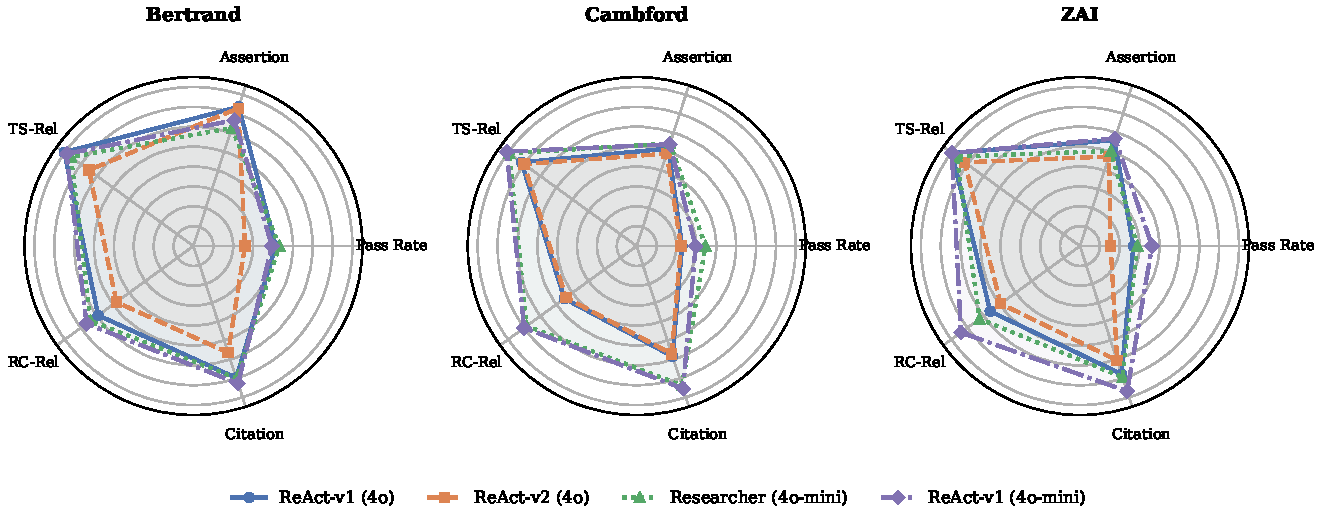
\includegraphics[width=\linewidth]{figures/agent_radar.pdf}
\caption{Per-tenant agent profiles. Each subplot shows the three agents on a shared radar for one tenant. On Bertrand (dense, small) all agents overlap; on Cambford (temporal multi-hop) \textsc{Researcher}'s citation and pass-rate advantage widens; on ZAI (large, bursty) \textsc{ReAct-v1} matches or exceeds the planner on assertion accuracy.}
\label{fig:agent_radar}
\end{figure}

\subsubsection{Query-Type Analysis}
\label{sec:query-type-analysis}

The evaluation set comprises three query categories generated with a 40/40/20 target split: \emph{fact-check} (single-entity retrieval), \emph{multi-hop} (cross-artifact reasoning), and \emph{report} (multi-source synthesis). Breaking down assertion and citation metrics by query type reveals how each architecture handles increasing retrieval complexity.

\begin{figure}[h]
\centering
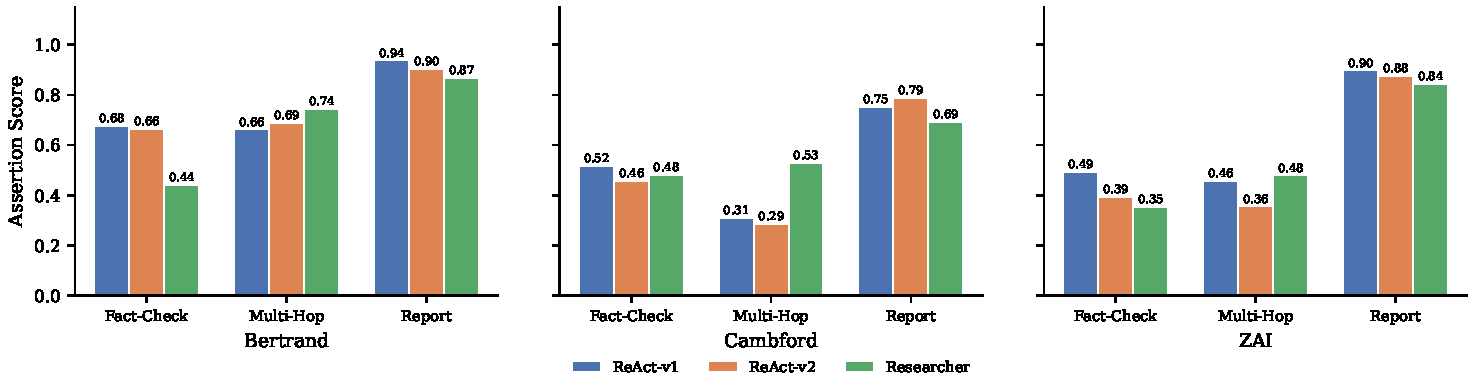
\includegraphics[width=\linewidth]{figures/assertion_by_query_type.pdf}
\caption{Mean assertion score by query type and tenant. All agents perform best on fact-check queries. The gap between agents widens on multi-hop and report queries, where \textsc{ReAct-v1}'s precision advantage is most pronounced.}
\label{fig:assertion_by_query_type}
\end{figure}

\begin{figure}[h]
\centering
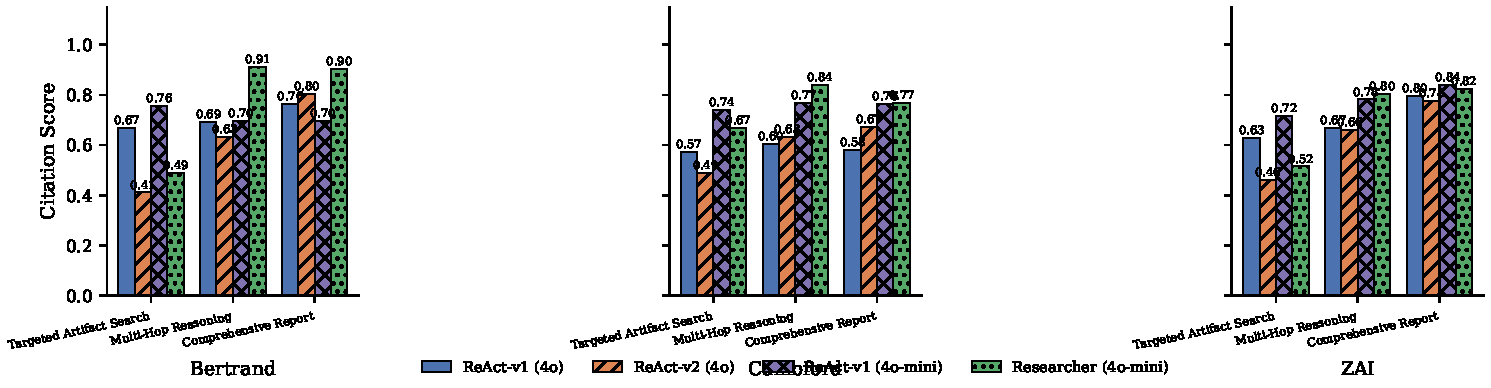
\includegraphics[width=\linewidth]{figures/citation_by_query_type.pdf}
\caption{Mean citation score by query type and tenant. \textsc{Researcher} leads on report queries where its planning stage systematically covers multiple source types, while the reactive agents are competitive on fact-check queries.}
\label{fig:citation_by_query_type}
\end{figure}

\begin{figure}[h]
\centering
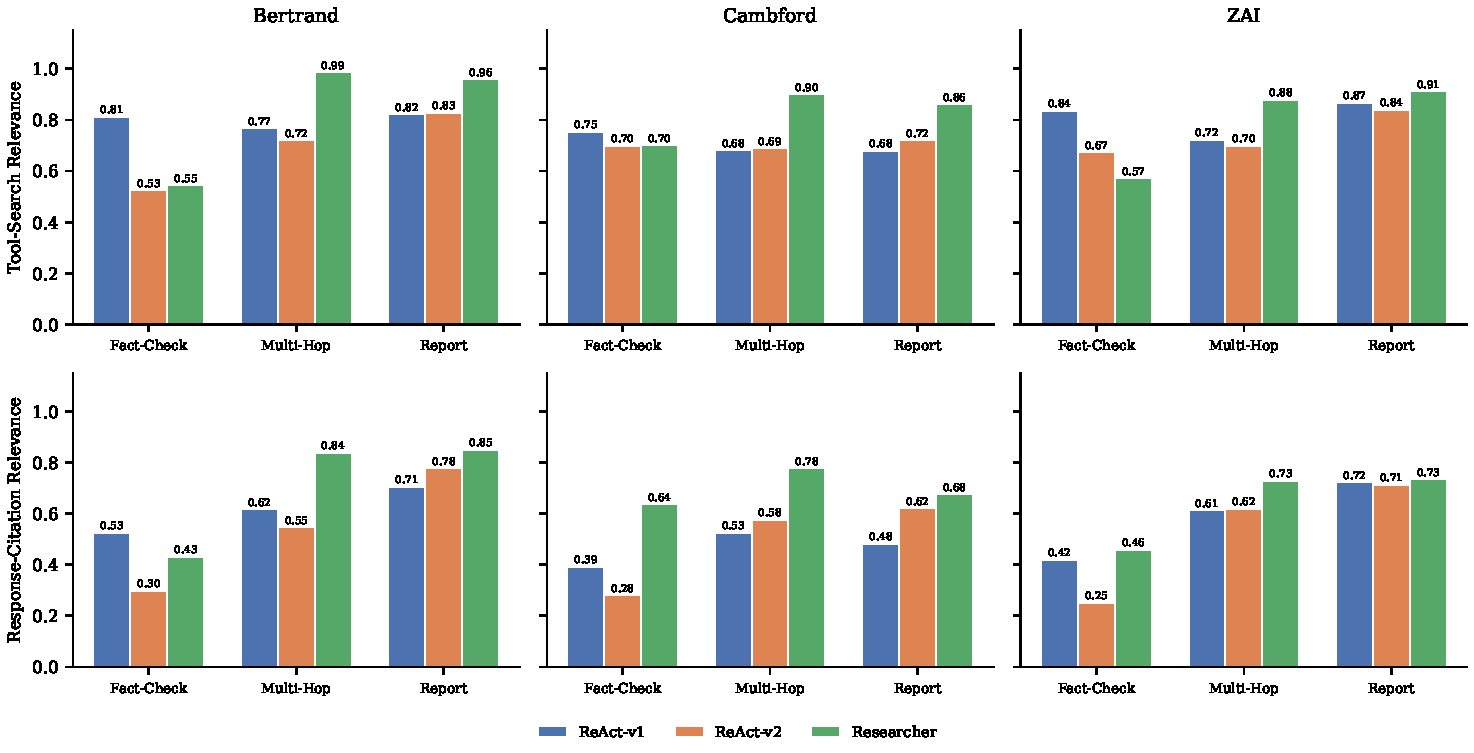
\includegraphics[width=\linewidth]{figures/citation_decomp_by_query_type.pdf}
\caption{Citation decomposition (tool-search relevance and response-citation relevance) by query type. Top row: tool-search relevance; bottom row: response-citation relevance. The performance gap between agents is most visible on report queries, where \textsc{Researcher}'s broader retrieval strategy produces higher relevance across both sub-metrics.}
\label{fig:citation_decomp_by_query_type}
\end{figure}

\noindent On fact-check queries, which require locating a single artifact, all three agents achieve their highest assertion scores and the inter-agent gap is narrow. This confirms that when evidence is concentrated in a single entity, even a minimal reactive loop suffices. On multi-hop queries, assertion scores drop across the board as agents must connect information across multiple artifacts; here \textsc{ReAct-v1}'s detailed worked examples help it maintain higher per-assertion accuracy than \textsc{Researcher}, whose broader retrieval introduces noise. On report queries, \textsc{Researcher}'s planning stage provides the clearest advantage in citation quality: its dependency-chain decomposition ensures that multiple source types are systematically retrieved and cited, while the reactive agents struggle to organize comprehensive responses from ad-hoc retrieval sequences.

\subsubsection{Cost–Effectiveness Trade-off}
\label{sec:cost-tradeoff}

The results reveal a clear cost-effectiveness frontier. \textsc{Researcher} achieves the highest pass rate (35.5\%) and citation quality (0.711) but consumes $5.2\times$ more prompt tokens (92{,}280 vs.\ 17{,}778) and $3.7\times$ more wall-clock time (65.2\,s vs.\ 17.6\,s) than~\textsc{ReAct-v1}. For deployments where retrieval completeness and citation traceability are the primary objectives---legal research, compliance auditing, or due-diligence workflows---this overhead may be justified. For latency-sensitive applications or scenarios with dense, recent evidence, \textsc{ReAct-v1} provides 32.3\% pass rate at $3.7\times$ lower latency with higher factual precision (assertion 0.638 vs.\ 0.557).

\textsc{ReAct-v2} does not occupy a Pareto-optimal point on this frontier: it matches \textsc{ReAct-v1} on tool-call count (1.70) and is marginally faster, but lags on all quality metrics. This finding suggests that prompt compression is costly in the absence of compensating architectural changes---a concise prompt is not equivalent to an equally effective one.

\begin{figure}[h]
\centering
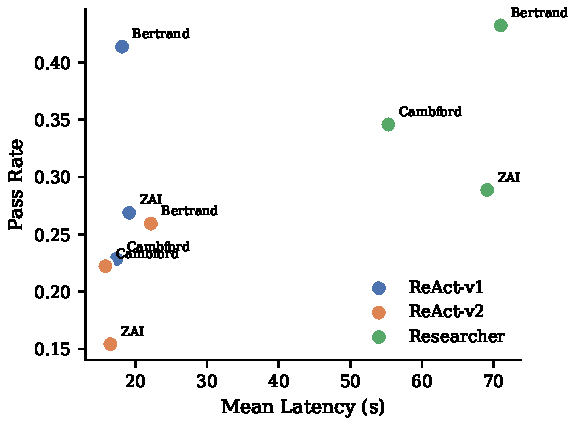
\includegraphics[width=0.75\linewidth]{figures/latency_vs_pass.pdf}
\caption{Latency--quality trade-off: mean wall-clock time vs.\ pass rate. \textsc{Researcher} occupies the high-latency/high-quality quadrant while the two reactive agents cluster at low latency; \textsc{ReAct-v1} achieves $3.7\times$ lower latency than \textsc{Researcher} with only a modest pass-rate gap.}
\label{fig:latency_vs_pass}
\end{figure}

\begin{figure}[h]
\centering
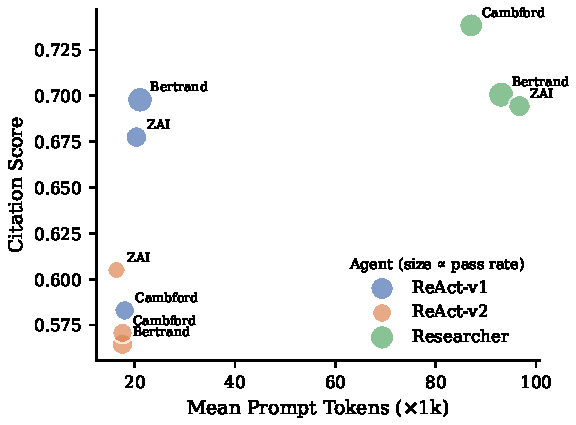
\includegraphics[width=0.7\linewidth]{figures/cost_quality_frontier.pdf}
\caption{Cost--quality frontier: mean prompt tokens vs.\ citation score. Marker size is proportional to pass rate. \textsc{Researcher} achieves the highest citation quality at $5.2\times$ the token cost of the reactive agents; \textsc{ReAct-v2} does not occupy a Pareto-optimal point.}
\label{fig:cost_frontier}
\end{figure}
